\documentclass[heading.tex]{subfiles} 
\begin{document}

\section{Introduction}

Hyperloop is a conceptual transportation system designed to lower costs and travel times relative to California’s current high-speed rail project.
\cite{Musk} Elon Musk and a team of engineers from Tesla Motors and the Space Exploration Technologies Corporation (SpaceX)
proposed the idea in August 2013, as an open design to be vetted and further refined through public contribution.
The concept deviates from existing high-speed rail designs by eliminating the rails, enclosing the passenger pod in a 
tube under a partial vacuum, and suspending the pod on air bearings. Propulsion is handled by a set of linear 
electromagnetic accelerators mounted to the tube, with the entire system being held above ground on concrete 
columns maintaining a straight trajectory.

\begin{figure}[hbtp]
\centering
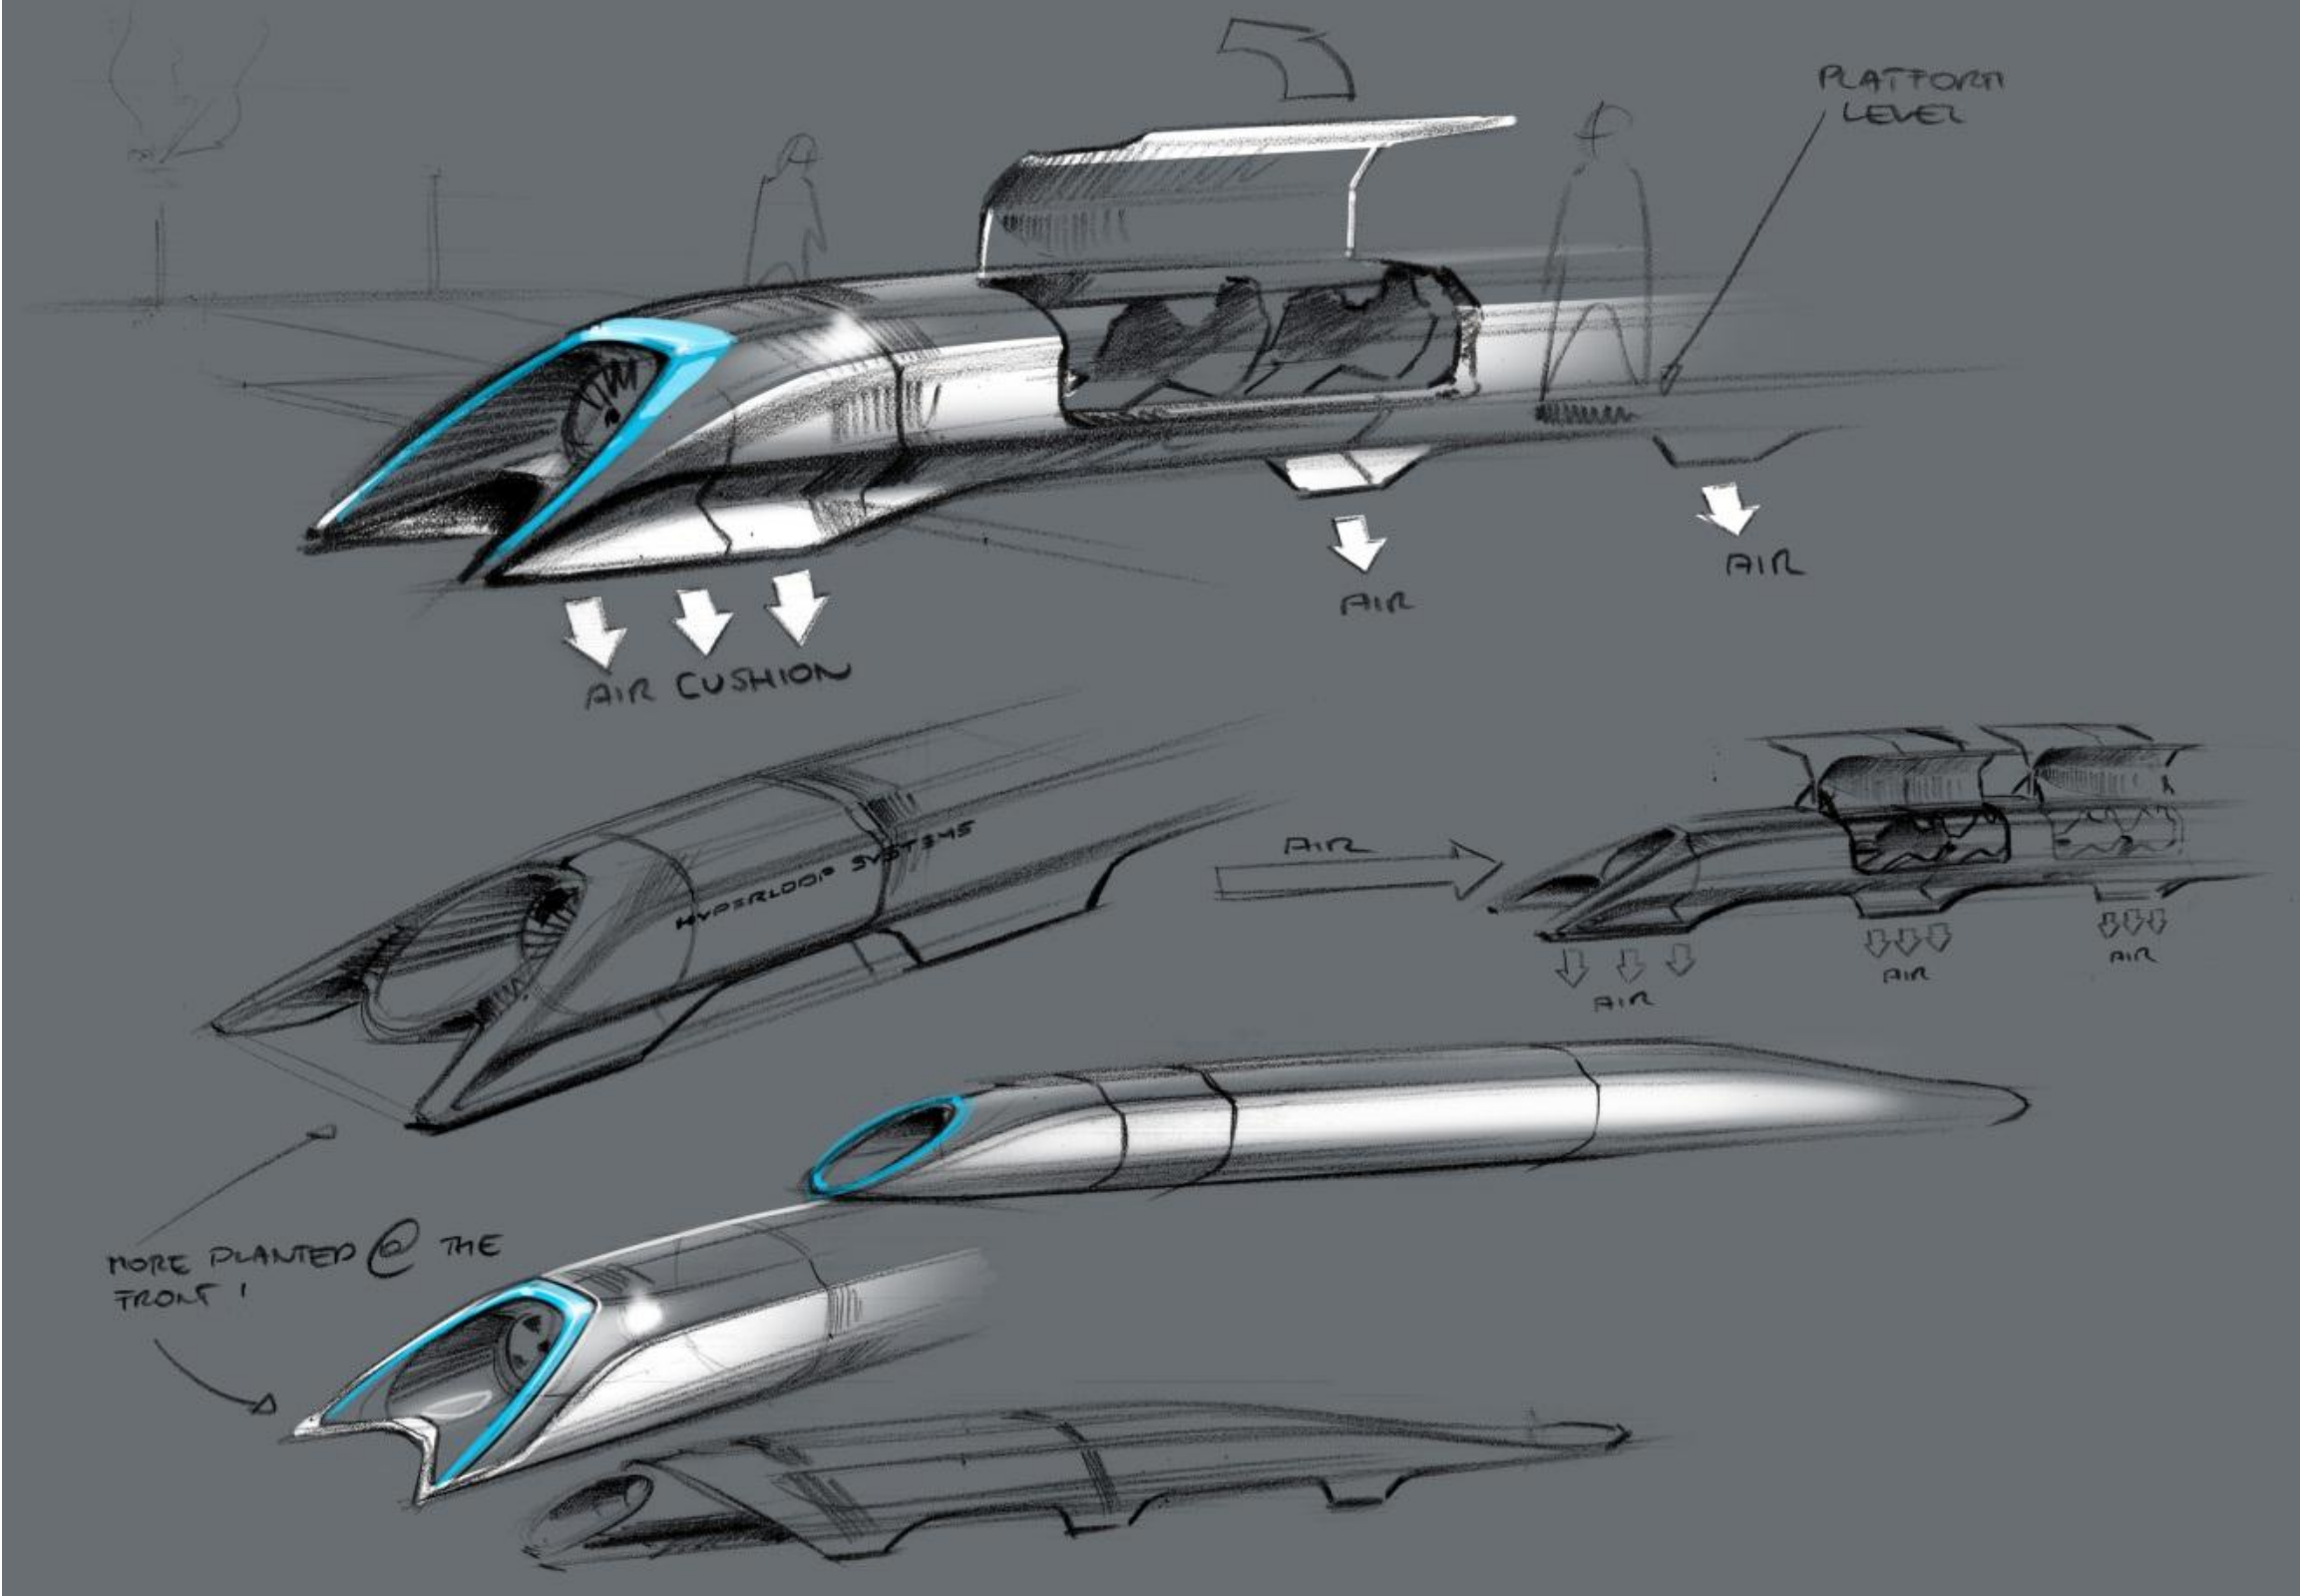
\includegraphics[width=.75\textwidth]{images/hyperloopAlphaSketch.png}
 \caption[Hyperloop Concept Sketch]{Hyperloop-alpha concept sketch of the passenger pod. \cite{Musk}}
\label{f:hyperloopSketch}
\end{figure}

Although Hyperloop is similar to other vacuum tube train (VacTrain) concepts \cite{ET3}, the soft vacuum represents a distinct difference.
It allows the train to run on air-bearings, thus removing the need for a magnetic levitation system used on the other VacTrain concepts.
The air bearings require a source of pressurized air, which is provided by an electric compressor system powered by on-board batteries.
Because Hyperloop operates in an atmosphere, it has many unique issues that need to be modeled as part of its sizing analysis. 
The modeling approach applied here is inspired heavily by methods for aircraft sizing and turbine engine cycle analysis. Hyperloop 
operates at transonic Mach numbers in a low pressure environment, so it is fairly strait forward to make the analogy to aircraft. 
The compression subsystem on the passenger pod is similar to the compressors on an aircraft engine. The aerodynamic concerns  
regarding the flow through the travel tube are essentially the same as those for the inlet of an aircraft engine. 

Musk’s original Hyperloop proposal included individual high-level analyses of many major subsystems including the pod compression system,
elevated support structure, and propulsion system. While this demonstrated the basic viability of the concept, it did not address
significant interdisciplinary couplings inherent in the Hyperloop system. These couplings introduce certain constraints which limit the 
degrees of freedom available in the design space. The major contribution of this work was to identify the key couplings that constrain the design space
and adapt methods from aircraft design to construct a conceptual design process that accounts for them. The most significant 
interdisciplinary coupling arose between passenger pod size and travel tube size. Because of aerodynamic concerns it was not possible to vary 
both pod size and tube size independently of each other. An additional, though less severe, coupling arose between the compression system and 
the thermal management system. All of the interdisciplinary coupling demanded the use of an iterative sizing procedure that balanced 
all the various systems to provide a feasible design for any given set of design variables. The results of this sizing process show that
the Hyperloop concept is feasible, but certain estimates from the original proposal may have been overly optimistic. 

This sizing process presented here was a necessary precursor step before ultimately performing a design optimization of 
Hyperloop with the dual objectives of minimizing ticket cost and travel time. Performing this optimization 
was outside the scope of this work and is reserved for future investigation. 
The fully integrated system model was constructed using OpenMDAO, a Python based framework for 
the design and optimization of complex systems\cite{GrayBenmarking2013}. The models presented 
in this work represent very basic analyses which rely heavily on simplifying assumptions. A realistic design 
optimization will require more detailed models of the investigated systems and additional analyses for economic models and 
structural models. Adding all of this will result in significant growth in complexity of the Hyperloop model. 
OpenMDAO could provide the means to manage growing model complexity 
in an efficient and flexible manner. Musks original work was released with the stated goal of jump starting
a crowd sourced design effort. In that spirit all the analyses used in this work have been released under
the Apache V2.0 open source license so that they could potentially serve as a foundation for future work.


\begin{figure}[hbtp]
\centering
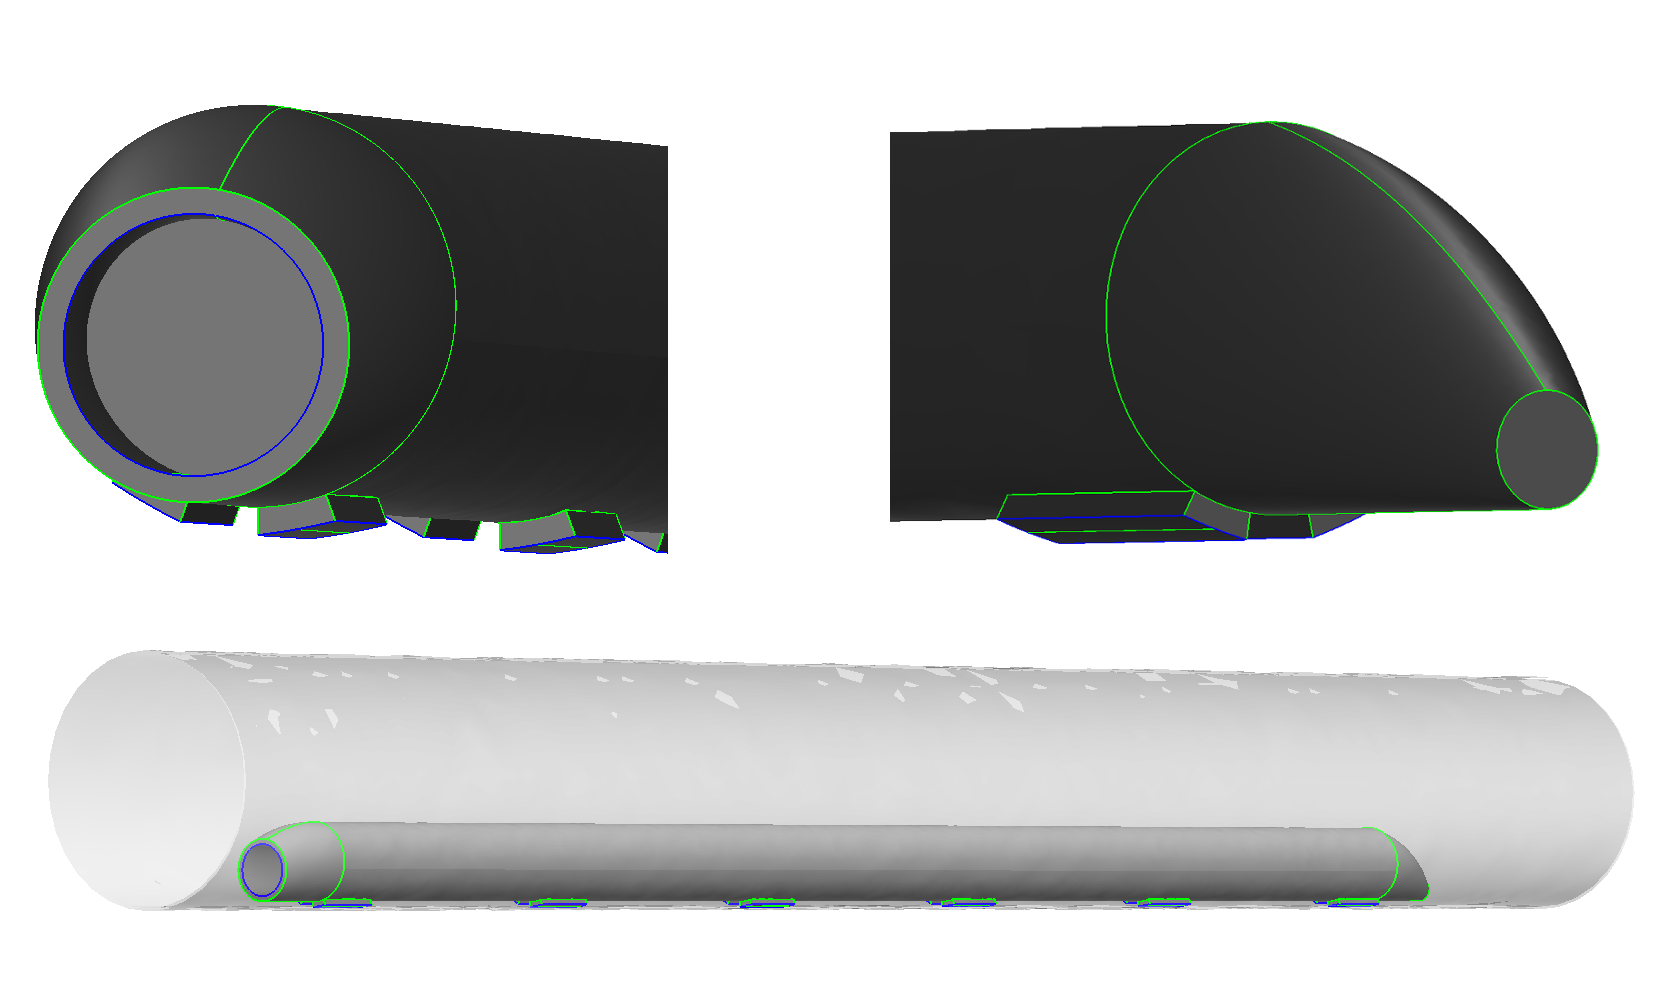
\includegraphics[width=\textwidth]{images/hyperloop_cad.png}
 \caption[Hyperloop geometry assembled in OpenCSM]{Calculated baseline inlet (left), nozzle (right), and full assembly (bottom) for a pod speed of Mach 0.8. Geometry rendered in OpenCSM, a parametric solid modeling tool.}
\label{f:hyperloopCAD}
\end{figure}


\section{Hyperloop Model Structure}

% A large interdependence between the various Hyperloop subsystems stem
% from design variables dictated by the tube and passenger pod systems.
% This coupling, along with other feedback relationships discussed later, require an
% iterative approach to arrive at a physically valid state for the entire system.

The Hyperloop passenger pod was decomposed into 5 primary analyses that were connected to 
form the conceptual sizing model. 

\begin{enumerate}
  \item Compression System: Performance and power consumption of the compressors.
  \item Mission Analysis: Estimate of travel time and velocity profile.
  \item Pod Geometry: Physical dimensions of the passenger pod.
  \item Tube Flow Limitations: Pod speed limitations based on choked flow restrictions.
  \item Tube Wall Temperature: Equilibrium temperature of the tube.
\end{enumerate}

The relationship between the systems is illustrated in figure \ref{f:hyperloopXDSM}. Feed forward connections 
are represented as the blue arrows in the upper right side of the diagram. For example, the Compressor Cycle 
passes data to the Mission Analysis, Pod Geometry, and and Tube Temperature analyses. In the lower left 
side of the diagram red arrows represent feed back connections which establish coupling between different 
analyses. 

\begin{figure}[hbtp]
\centering
\includegraphics[width=\textwidth]{images/TopAssembly.png}
\caption{Workflow and dependencies between the major Hyperloop subsystems.}
\label{f:hyperloopXDSM}
\end{figure}

The compression system and pod geometry analyses were each further subdivided into a number of subsystems. The pod geometry 
system was primarily responsible for computing important areas throughout the passenger pod. Figure \ref{f:podXDSM} shows the 
pod geometry breakdown into 5 subsystems. Most of these calculations were based on simple geometric relationships. The 
modeling was broken down to enhance modularity so that future work could replace these simple analyses with more advanced ones. 

\begin{figure}[hbtp]
\centering
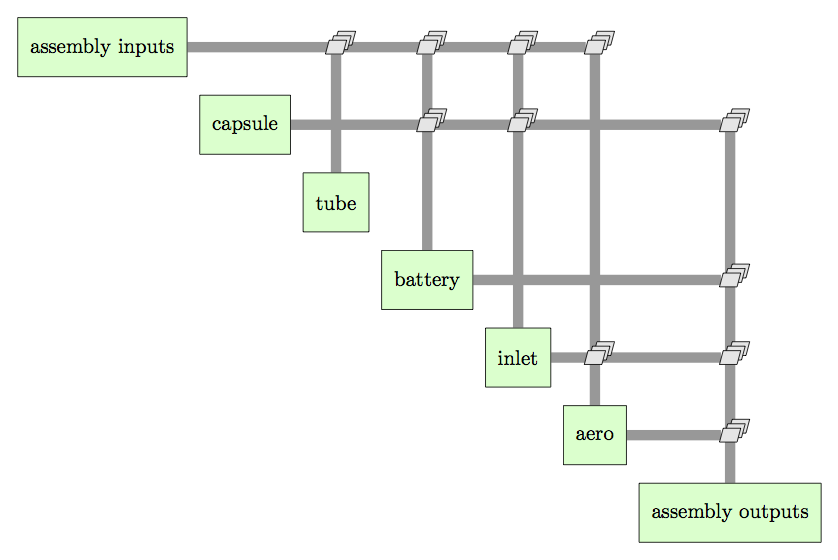
\includegraphics[width=0.7\textwidth]{images/pod_assembly_xdsm.png}
\caption{Expanded \texttt{pod} assembly XDSM}
\label{f:podXDSM}
\end{figure}

The compressor cycle performed calculations related to the thermodynamic processes associated with compressing, cooling, and exhausting air. 
The modeling approach for the compressor cycle was heavily influenced by techniques developed in the Numerical Propulsion System Simulation (NPSS) code. 
NPSS was created as a joint effort between United States engine manufacturers and NASA Glenn Research Center for the purpose of 
simulating and analyzing turbomachinery cycles for aircraft applications\cite{Lytle}. NPSS employs a highly modular model construction
where cycles get broken down into individual thermodynamic processes and then connected together. This modularity was adopted for pyCycle, 
the cycle modeling tool used in this work. 

\begin{figure}[H]
\centering
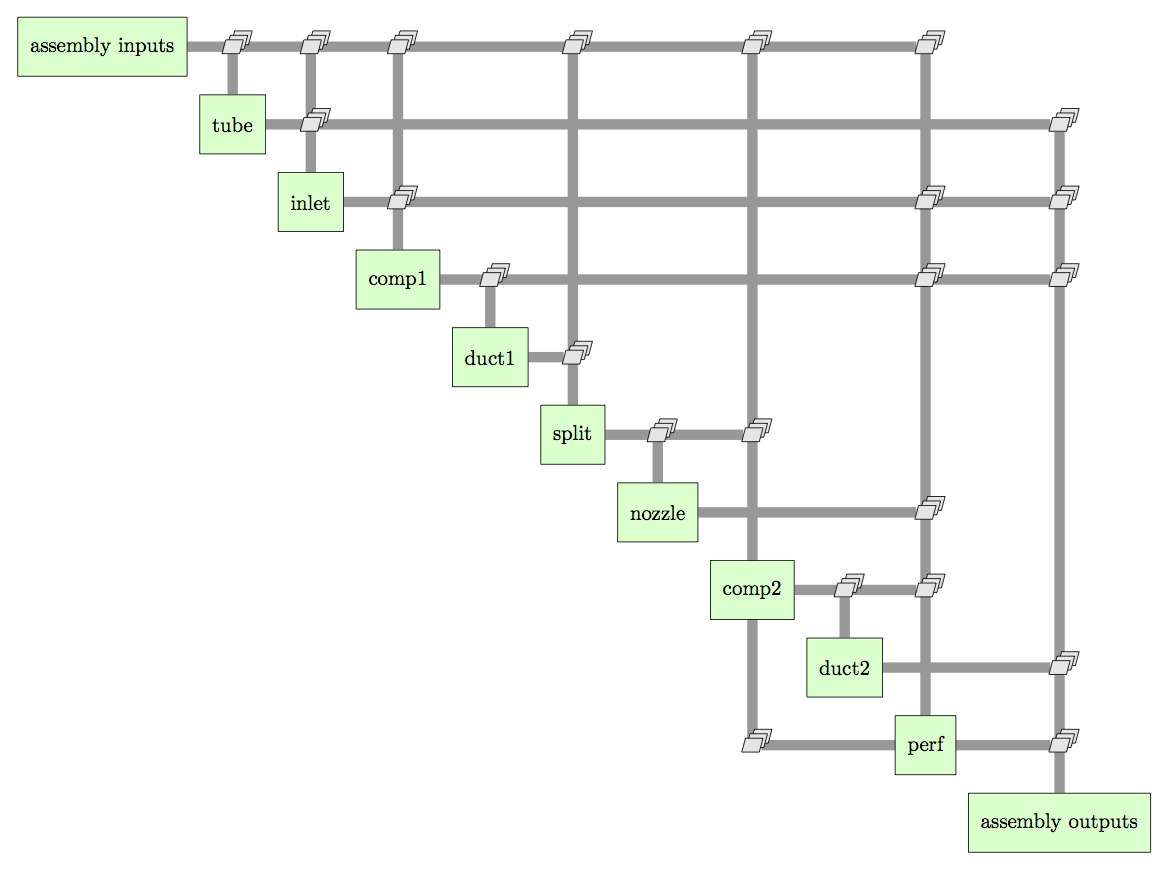
\includegraphics[width=0.85\textwidth]{images/compress_assembly_xdsm.png}
\caption{Expanded \texttt{compress} assembly XDSM}
\label{f:compressorXDSM}
\end{figure}

\section{Pod and Tube Sizing}

These couplings enforce a set of equality constraints that must be satisfied for any physically valid Hyperloop design.
A solver is necessary to perturb numerous design and state variables to characterize the system of equations and drive
each variable towards a specified valid criteria. The first equality constraint requires agreement between the pod geometry
calculations and the computed compression system areas. The second constraint ensures the pod compressor achieves the
necessary flow intake given a maximum bypass flow, and the final feedback loop drives the operating tube temperature to
balanced conditions. Figure \ref{f:hyperloopXDSM} only shows the highest level assembly connections;
the compression system and pod geometry system are further expanded into sub-assemblies in \cref{app:model}.
The feedback loop between the tube and inlet diameter is more severe than described in the original proposal,
which can be explained with a closer examination of the coupled geometries and mass flow rates.

\begin{figure}[hbtp]
\centering
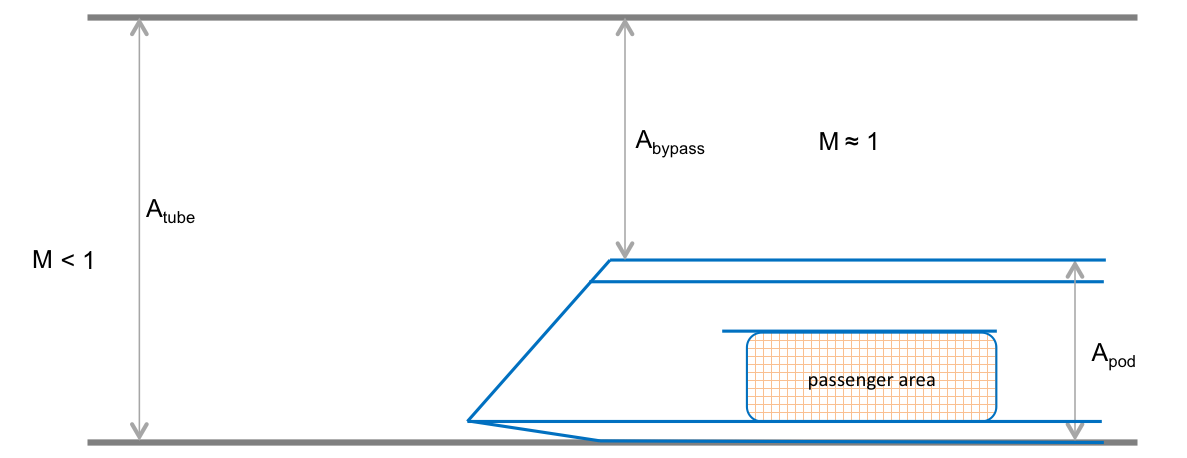
\includegraphics[width=\textwidth]{images/closedCapsule.png}
\caption{Longitudinal view of a passenger pod with no inlet and compression system.}
\label{f:ClosedPod}
\end{figure}

Figure \ref{f:ClosedPod} shows the most simplified case of an enclosed pod with no inlet.
In this scenario, the air reaches the pod at a relative velocity equal to the pod speed
and accelerates as it is forced through the smaller bypass area around the pod.
Assuming a circular cross section for both the pod and tube, the bypass air must travel through an area given by

\nomenclature{A}{Area (m^{2})}
\nomenclature{r}{Radius (m)}
\begin{equation*}
A_{bypass} = \pi(r_{tube}^2-r_{pod}^2)
\end{equation*}
\nomenclature{\rho_}{Density (\frac{kg}{m^{3}})}
\nomenclature{\dot{W}, \dot{m}}{Mass Flow Rate (kg/s)}

Since $A_{tube}$ and the air density $\rho_{air}$ are both constant for given tube size, then the mass
flow rate of the air traveling around the pod ($\dot{W}_{bypass}$) grows linearly with the velocity of the pod.

\nomenclature{V}{Velocity ($\frac{m}{s}$)}
\begin{equation*}
\dot{W}_{bypass} = \rho_{air} A_{tube} V_{pod}
\end{equation*}

However, the flow reaches a physical limitation as it approaches the speed of sound. At this point, no additional flow can escape
around the sides of the vehicle without increasing the density of the air.
For a given area ratio, the limiting pod speed can be determined based on isentropic flow relations, where $\gamma$ is the heat capacity ratio.

\nomenclature{\gamma}{Heat Capacity Ratio}
\nomenclature{MN}{Mach Number}
\begin{equation*}
\frac{A_{tube}}{A_{bypass}} = \left(\frac{\gamma+1}{2}\right)^{-\frac{\gamma+1}{2\left(\gamma-1\right)}}\frac{\left(1+\frac{\gamma-1}{2}MN^{2}\right)^{\frac{\gamma+1}{2\left(\gamma-1\right)}}}{MN}
\end{equation*}

\begin{figure}[hbtp]
\centering
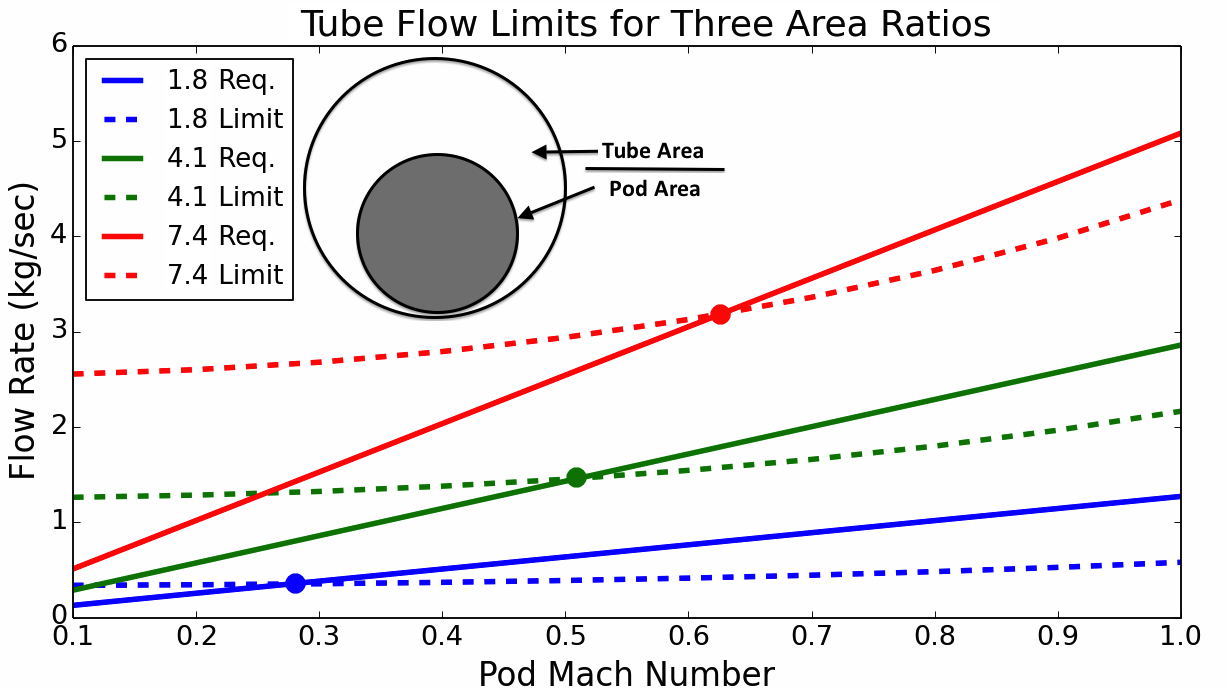
\includegraphics[width=\textwidth]{images/tube_flow_limit3.png}
\caption{Hyperloop speed limits as a function of three different area ratios}
\label{f:flowLIMIT}
\end{figure}

This limiting pod speed can be visualized by the intersecting lines in figure \ref{f:flowLIMIT} for three different area ratios.
The solid lines represent the required bypass flow rates necessary for a given speed,
and the dashed lines signify the flow limit, which is bounded by a sonic condition around the sides of the pod.


To further increase speeds, an inlet and compression system is needed to help draw additional air through the pod.
The vertical distances between the dashed lines and solid lines of figure \ref{f:flowLIMIT} correlates to the
minimum compressor flow rates necessary to achieve a given speed. 

\begin{figure}[hbtp]
\centering
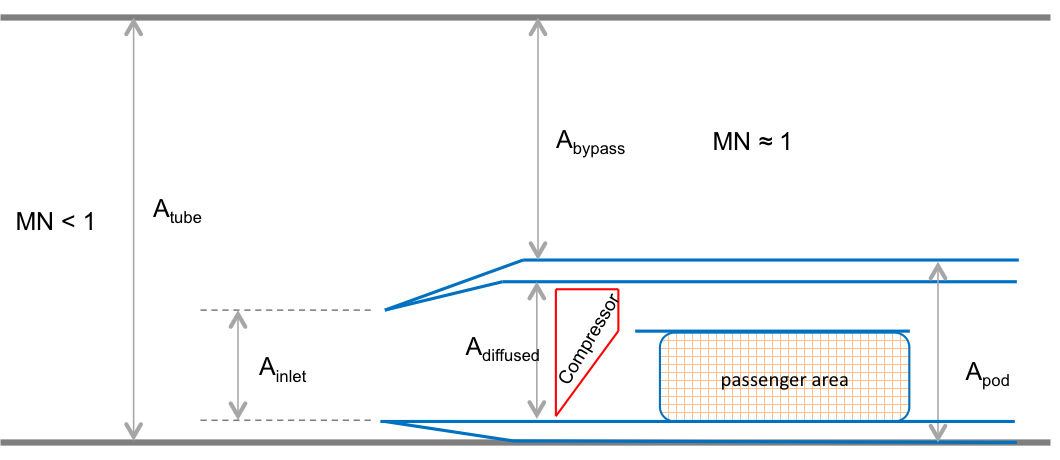
\includegraphics[width=0.85\textwidth]{images/openCapsule.png}
\caption{Longitudinal view of a passenger pod with a simplified inlet and compression system.}
\label{f:OpenPod}
\end{figure}

By integrating a ducted compression system into the passenger pod, as shown in figure \ref{f:OpenPod},
higher mass flows can be passed through the vehicle than can be forced around the sides.
This system would require an inlet that diffuses air before reaching the compressor fan face,
further increasing the cross sectional area of the pod.
Part of the compressed air would support the air bearings, with the remainder accelerated out a nozzle aft of the pod.
Additional non-linearity is introduced when considering the limitations of the compressor system.
Increased speeds either necessitate a larger compressor diameter to sufficiently diffuse incoming air,
or the compressor needs to be designed to handle increased flow demands.
Increased speeds also necessitates a larger tube to pod area ratio as depicted earlier.

\nomenclature{c1MN}{Mach number at the front face of the first compressor}
\begin{figure}[H]
\centering
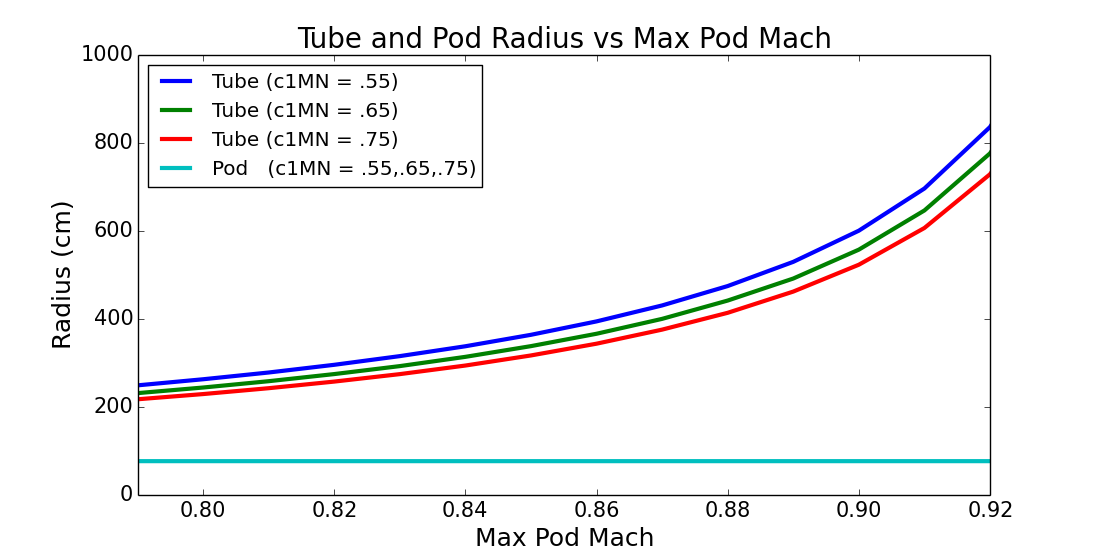
\includegraphics[width=\textwidth]{images/mach_vs_rad4.png}
\caption[Tube and Pod Radius vs Mach]{Exponential relationship between pod speed and required tube radius, for three diffused mach numbers.
Converged pod radius also show underneath. }
\label{f:machRAD}
\end{figure}

The compounding relationship of a growing pod area, and a growing area ratio is
shown in figure \ref{f:machRAD}, for three diffused mach numbers at the entrance of the first compressor(c1MN).
For each point on each curve, the full system model converges on the minimal possible tube diameter, given a desired pod Mach number.
This graph also accounts for compressor performance limitations and the steady-state operating tube temperature
that reaches quiescence above ambient conditions.
The absolute tube radius is charted rather than an area ratio as a more direct indicator of total system cost.
It's worth noting that the pod size is also free to vary at each point and is plotted on the cyan line.
Surprisingly, the pod radius remains nearly constant for every targeted speed condition.
This can be attributed to the sensitive nature of the inlet size when perturbed in either direction.
Decreasing the inlet diameter prohibits airflow through the capsule to a greater extent than it improves bypass air around the capsule,
due to the squared radius term determining the areas.
The inlet area is also bounded by necessary flow requirements for the bearings and volume requirements of the passenger cabin.

Without a ducted capsule, the proposed pod and tube dimensions would allow a max speed of around 120 $\frac{m}{s}$, or Mach 0.3.
Such low speeds would not allow the Hyperloop concept to significantly reduce travel times between Los Angeles
and San Francisco relative to high speed rail.
Adding a compression system and doubling the diameter of the tube would allow the pod to reach speeds closer to Mach 0.8.
At these speeds, the estimated travel time is closer to 40 minutes, following the velocity profile
necessary to reduce acceleration around banked turns.
Although this performance is much less favorable than that described in the original proposal,
it still provides a compelling case when compared to high speed rail. 
The compressor system necessary to achieve this performance is analyzed next.

\section{Compressor Power and Battery Sizing}
\label{sec:compressor-and-battery}

The on-board compression system serves dual purposes.
It provides a means of exceeding the nominal Kantrowitz limit and also supplies pressurized air to support the air bearing system.
Each of these functions requires a minimum airflow to rise to a specified pressure gain,
and combine to define the total airflow requirements of the subsystem.
The subsequent thermodynamic analysis of the compressor system is also necessary to
estimate on-board power requirements and overall heat rise of each pod.
The compression cycle is comprised of an inlet, two compressors, a nozzle, and multiple ducts leading to air bearings.
The design deviates from the original proposal by removing two heat exchangers for reasons explained in the following section.
The system, shown in figure \ref{f:comp} is modeled as a one dimensional cycle,
representing components as thermodynamic processes that are subsequently chained together.
Each component is responsible for calculating gas properties across its boundaries
and appropriately enforcing conservation equations across the entire system.

\begin{figure}[hbtp]
\centering
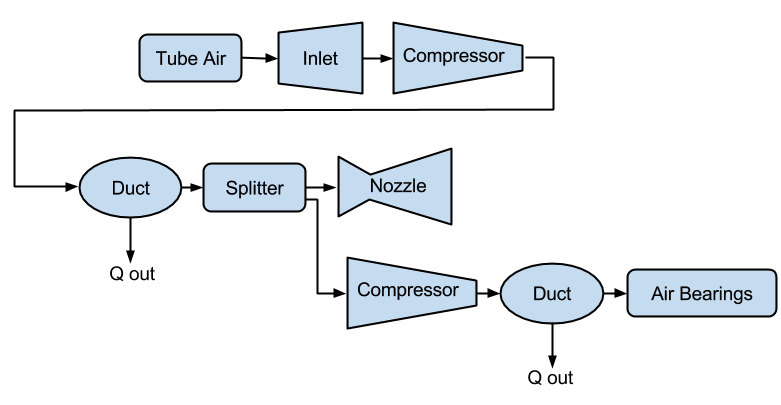
\includegraphics[width=0.9\textwidth]{images/compressor_schematic.png}
\caption{Schematic flow diagram of the modeled compressor system}
\label{f:comp}
\end{figure}

The simulation leverages the Numerical Propulsion System Simulation (NPSS) code, which
was created as a joint effort between United States engine manufacturers and NASA
for the purpose of simulating and analyzing thermodynamic processes, particularly turbomachinery cycles. \cite{Lytle}
The model was then adapted to pyCycle, an open-source cycle analysis tool that employs Cantera for thermodynamic calculations.
Further information on these tools can be found in the appendix and online documentation. \cite{goodwin2009cantera}

These models predict the instantaneous power consumption of the compressors, temperature and pressure rises,
and upstream conditions necessary to supply sufficient airflow to the bearings.
These power requirements are a function of the chosen cycle and are both affected by
and contribute to the thermal conditions, creating the feedback loop “C” in figure \ref{f:flowLIMIT}.
Combined with the mission profile described below, these requirements impact battery sizing.

\begin{figure}[hbtp]
\centering
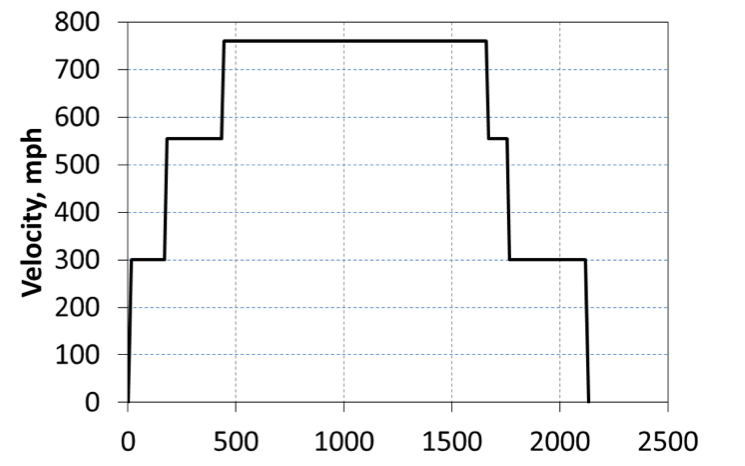
\includegraphics[width=0.7\textwidth]{images/velocity_profile.png}
\caption{Velocity profile described in the original proposal}
\label{f:velocity}
\end{figure}

Using the notional velocity profile described in the original proposal, and shown in figure {ref},
a speed factor can be estimated by normalizing the profile then scaling it based on the maximum
attainable velocity calculated in the previously discussed subsystems.
From the resulting speed factor, or ratio of average speed to maximum speed,
a crude estimate of total travel time can be deduced based on total tube length.
Multiplying this time by the average compressor power consumption and a 30\% safety margin results in an overall battery storage requirement.

\begin{figure}[hbtp]
\centering
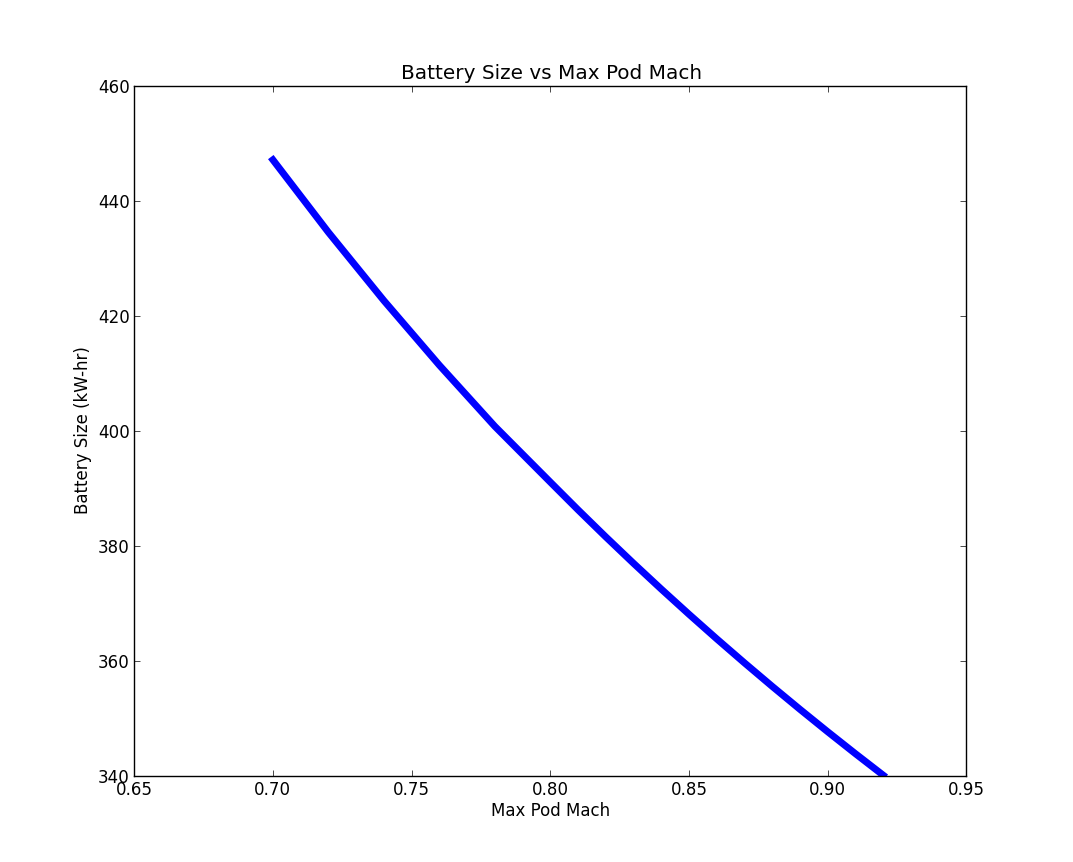
\includegraphics[width=0.8\textwidth]{images/mach_vs_energy.png}
\caption[Battery requirements as a function of pod speed]{Battery requirements as a function of pod speed. Note: the y-axis begins at 340kW-hr.}
\label{f:battery}
\end{figure}

The necessary on-board battery size was found to be inversely related to the max pod speed, as shown in figure \ref{f:battery}.
This indicates that compressor power requirements are less sensitive to increased speeds than total trip time.
Although traveling at higher speeds draws more energy, the system is operated for a shorter period of time.
This sensitivity is highly dependent on the velocity profile.
Therefore, reducing time spent at max speed could result in a positive correlation between battery size and pod speed.
It should also be noted that the Y-axis of figure \ref{f:battery} begins at 340kW to emphasize the downward trend.
The overall reduction in battery size is on the order of 25\%, if speed is increased from Mach 0.7 to Mach 0.9.
Additional mission analysis details can be found in \cref{app:route} and work done by Mathworks \cite{Rouleau}.
These estimates are in agreement with Musk’s work, and equate to roughly 3 to 5 battery packs from a Tesla Model-S.
However, the estimates are still optimistic since no work has been done to estimate battery cooling requirements,
and based on the assertion that the compression cycle does not need to be cooled.
The system-level thermal interactions and heat exchangers are analyzed next.

\section{Heat Exchanger and Tube Thermal Analysis}

As each pod passes through the tube, it adds energy to the air in the form of heat.
Following the proposed frequency of launching a pod every six minutes,
the continuous operating cycle could potentially heat the overall tube to excessive temperatures.
To combat this effect, the original proposal recommends a heat exchanger that would be integrated into the compression system.
These intercoolers would use water stored in on-board tanks to cool the air and assist secondary compression.
The resulting steam could then be stored in a tank and offloaded once the pod reached its destination.
However, initial calculations show that using water for cooling is not an ideal design for two reasons:

1) The flow rate of water needed to remove the heat added by the compressors is very large, and the sheer volume constraints of storing
the resulting steam would outweigh the benefits.

2) The heat addition from each pod compressor cycle is fairly low relative to other heat transfer mechanisms occurring between the Hyperloop
and the external environment. Even without an active on-board cooling solution, the tube temperature would be dominated by other factors.

The following two sections provide additional details about the engineering models used to draw these conclusions.

\subsubsection{Pod Cooling Requirements}

The limits and requirements of a hypothetical on-board heat exchanger can be estimated with a straightforward energy balance. The
effectiveness of a heat exchanger can be described as the ratio of actual heat transfer over the maximum possible heat transfer.

\nomenclature{Q}{Heat flow rate (W)}
\begin{equation*}
{Q}_{released}  = effectiveness * {Q}_{max}
\end{equation*}


with $Qmax=\left(T_{hot,in} - T_{cold,in}\right) [ \dot{m} C_{p} ]_{fluid}$ where each fluid has a $\dot{m} C_{p}$ and the fluid with the lowest
product is used to determine the maximum heat transfer. In order to satisfy the energy balance $Q_{released}=Q_{absorbed}$ the following must be true,

\nomenclature{\dot{m}}{Mass flow rate}
\nomenclature{T}{Temperature (K)}
\nomenclature{C_{p}}{Heat capacity at constant pressure ($\frac{J}{kg-K}$) }
\begin{equation*}
\dot{m}_{air} C_{p, air} (T_{out, air} - T_{in, air}) = {Q}_{released} = {Q}_{absorbed}= \dot{m}_{water} C_{p,water} (T_{out, water} - T_{in, water})
\end{equation*}

where the $T_{out}$  of each fluid is unknown. With assumed mass-flow rates and initial temperatures, a valid combination of Tout‘s of
each fluid can be found through solver iteration. Valid effectiveness levels for heat exchangers can be estimated based on the
Effectiveness - Number of Transfer Units (NTU) method. 
The effectiveness for a counter flow heat exchanger with a $\frac{C_{p,min}}{C_{p,max}}$ of ~0.25 was chosen with air and water as the working fluids. 
The following conditions satisfied an energy balance with an extremely optimistically assumed effectiveness of 0.9765,
and the proposed requirement to fully cool the air back down to inlet temperatures.

\nomenclature{NTU}{Number of Transfer Units}

\begin{table} [H]
\centering
\begin{tabular}{|c|c|c|c|c|c|c|}
\hline 
Fluid & Cp & Tin & Tout & mdot & Q (kJ/s) & Qmax \\ 
\hline 
Air & 1.006 kJ/kh-K & 791 K & 300 K & 0.49 kg/s & -242 & 247.9 \\ 
\hline 
Water & 4.186 kJ/kg-K & 288.15 & 416.6 K  & 0.45 kg/s & 242 & 247.9 \\ 
\hline 
\end{tabular} 
 \caption{Heat Exchanger Fluid Properties}
\end{table}

With a 35 minute trip, $0.45 \frac{kg}{s} * 60 \frac{s}{min} * 35min = 945 kg$ of standard temperature/pressure water would need to be carried 
with steam tanks over a hundred meters in length. This doesn't even account for the second stage heat exchanger, making the system nearly infeasible
with water and unpressurized tanks. Various systems involving partial cooling, alternate coolants (such as liquid air), or pressurized tanks could be explored.

Further discussion of heat exchanger sizing can be found in the heat exchanger section of \cref{app:heatX}.
The calculations explore the possibility of multi-pass heat exchangers
and the logarithmic mean temperature difference (LMTD) of the heat exchanger is considered.
\cite{Cengal}
\cite{Turns}


\subsubsection{Equilibrium Tube Temperature}
A high-level assessment of the overall steady-state heat transfer between the 300 mile Hyperloop tube and the ambient atmosphere is
also investigated. The outer diameter of the pipe is chosen as the control surface boundary used in the heat balance. Heat added from the pod exhaust
air and solar flux are considered the primary drivers for heat absorption into the tube. Conversely, heat released from the tube is modeled by means of
ambient natural convection and radiation out from a stainless-steel surface. The thermal interaction between the rarified internal air and
tube is not modeled.

The heat being added by the pods can be determined from the cycle analysis, or based purely on inlet total temperatures with isentropic
flow relations.

\nomenclature{P}{Pressure ($\frac{N}{m^{2}}$)}
\nomenclature{PR}{Pressure Ratio}
\nomenclature{PR}{Pressure Ratio}
\nomenclature{{\eta}_{adiabatic}}{Adiabatic Efficiency}
\begin{equation*}
T_{t} = T_{s} * [1 + \frac{\gamma -1}{2} MN^2]
\end{equation*}
\begin{equation*}
P_{t} = P_{s} * (\frac{ T_{t}}{T_{s}})^(\frac{\gamma}{\gamma -1})
\end{equation*}
\begin{equation*}
P_{t,exit} = P_{t,inlet} * PR
\end{equation*}
\begin{equation*}
T_{t,exit} = T_{t,inlet} + \frac{([T_{t,inlet}*PR^{(\frac{\gamma-1}{\gamma})}] - T_{t,inlet})}  {{\eta}_{adiabatic}}
\end{equation*}

Where PR is the compressor pressure ratio, MN is the mach number,  $\gamma$ is the specific heat ratio, and  ${\eta}_{adiabatic}$ is the
adiabatic efficiency.

With the air flow rate known, the heat flow rate per pod is obtained,

\begin{equation*}
{Q}_{pod}= \dot{m}_{air} C_{p,air} (T_{out, air} - T_{tube})
\end{equation*}
The peak heating rate from the pods scales linearly.
\begin{equation*}
{Q}_{peak}= Q_{pod} (\# ofpods)
\end{equation*}
The solar heat flow per unit area can be approximated, given the solar reflectance index (SRI) of stainless steel, non-normal incidence factor
of the cylinder and solar insulation (SIF).

\nomenclature{SRI}{Solar Reflectance Index}
\nomenclature{SIF}{Solar Insulation Factor}
\nomenclature{{\theta}_{nni}}{Non-normal Incidence factor (rad)}
\nomenclature{L}{Length (m)}
\nomenclature{OD}{Outer diameter (m)}
\nomenclature{\epsilon}{Emissivity Factor}
\nomenclature{\sigma}{Stefan-Boltzmann constant ($\frac{W}{m-K}$)}
\nomenclature{P_{rad}}{Radiated Power (W)}
\nomenclature{L}{Length}

\begin{equation*}
Solar = (1-SRI) {\theta}_{nni} SIF
\end{equation*}
Multiplying this by the viewing area of the tube (assuming no shade and constant sun)
\begin{equation*}
Q_{solar} = Solar * A_{view} = Solar * L_{tube} * OD_{tube}
\end{equation*}
Tube cooling can be attributed to two general mechanisms, radiation and natural convection. Radiation power per unit area can be
approximated to
\begin{equation*}
\frac{P_{rad}}{A} = \epsilon \sigma (T_{pipe}^4 - T_{ambient}^4)
\end{equation*}
where  $\epsilon$ is the emissivity factor and  $\sigma$ is the Stefan-Boltzmann constant.

Multiplying by the surface area of the tube, the total heating rate can be found,
\begin{equation*}
Q_{rad} =  \frac{P_{rad}}{A} * \pi L_{tube} OD_{tube}
\end{equation*}

Assuming the worst case scenario of no cross wind, convection is primarily driven by temperature gradients. The non-dimensional relation
between buoyancy and viscosity driven flows is parameterized using the following empirical constants. \cite{Berton} \cite{Incropera}

if 150 K $<  T_{amb} <$ 400 K:

\nomenclature{g}{Acceleration of gravity, 9.81 ($\frac{m}{s^{2}}$)}
\nomenclature{\beta}{Volume coefficient of expansion (K)}
\nomenclature{\upsilon}{Kinematic Viscosity ($\frac{m^{2}}{s}$)}
\nomenclature{Pr}{Prandtl Number, $\frac{\upsilon}{\alpha}$}
\nomenclature{Gr}{Grashof Number, $\frac{ g \beta \delta TL^{3}}{v^{2}}$}
\nomenclature{Ra}{Rayleigh Number, $\frac{\rho U_{\infty} L}{\mu}$}
\nomenclature{Nu}{Nusselt Number, $\frac{hL}{k}$}
\nomenclature{h}{Heat transfer coefficient ($\frac{W}{m^{2}-K}$)}
\nomenclature{k}{Thermal Conductivity ($\frac{W}{m-K}$) }

\begin{equation*}
\frac{g \beta T} {\upsilon^2} =  4.178\times10^{19} \times T_{amb}^{-4.639}
\end{equation*}

\begin{equation*}
Pr = 1.23 T_{amb}^{-0.09685}
\end{equation*}

if 400 K $<  T_{amb}  <$ 2100 K:


\begin{equation*}
\frac{g \beta T} {\upsilon^2}  = 4.985\times10^{18} \times T_{amb}^{-4.284}
\end{equation*}
\begin{equation*}
Pr = 0.59 T_{amb}^{0.0239}
\end{equation*}
The Grashof Number can then be approximated,


\begin{equation*}
Gr = \frac{g \beta T} {\upsilon^2}  (T_{tube}-T_{amb}) {OD}_{tube}^3
\end{equation*}
The non-dimensional Rayleigh number can then be calculated to estimate buoyancy effects, leading to the Nusselt number.


\begin{equation*}
Ra = Gr * Pr
\end{equation*}
\begin{equation*}
Nu = \Bigg(0.6 + \frac{0.387Ra^{\frac{1}{6}}}{[1+(\frac{0.559}{Pr})^{\frac{9}{16}}]^{\frac{8}{27}}}\Bigg)^2
\end{equation*}

From this point the total heat transfer from natural convection can be obtained,

\begin{equation*}
Q_{nat. conv} = hA \Delta T = \frac{k*Nu}{ {OD}_{tube}} \pi {L}_{tube} {OD}_{tube} (T_{tube}-T_{amb})
\end{equation*}

The steady state tube temperature can be found by varying the tube temperature until the rate of heat being released from the tube
matches the rate of heat being absorbed by the tube.
Assuming numerous state variables provided in the source code, a steady state temperature of 120 F was reached.
This result suggests that there is no need for on-board cooling, however many baseline assumptions have yet to be validated or even defined.

\section{Conclusions}



For the most part, the ideas and numbers given in the original Hyperloop proposal hold up using this analysis. However, the data shows that
there are two major changes to the design that need to be considered.
The tube cross section will need to be significantly larger than the original proposal. In the original proposal, the tube was sized with a diameter 2.23
meters. However, it appears that it will need to have a diameter closer to 4 meters to reach speeds maximum speeds of Mach 0.8.
On-board water based inter-coolers also seem impractical due to both volume and weight constraints. This may prove to be a non-issue since
temperature rise due to compression is significant less than originally estimated and only leads to a modest rise in steady-state tube
temperature. Assuming the tube was left uncovered, the heat rate from solar radiation would be an order of magnitude larger than the heat
rate added from pod compression systems. Further assuming a 90 degF day, radiation and convection out of the tube would lead to a
manageable steady state tube wall temperature of 120 degF.

Current tool-sets provide sufficient complexity management, however a larger breadth of disciplines need to be modeled before ultimately
understanding the feasibility of this unique multidisciplinary problem.

\end{document}
